\section{Relations Groupes/Sessions}

Pour éclaircir les concepts de groupes de processus et de sessions, examinons l'exemple de code shell ci-dessous, offrant une opportunité pratique pour illustrer leur interaction.

\begin{lstlisting}[style=blackstyle]
$ echo $$ # PID du shell
1121
$ yes "data" | head -n 10000000000 > /dev/null &  # 2 process en background
[1] 1147
$ ps -o "pid,ppid,pgid,sid,cmd" # 1 process en foreground
  PID    PPID    PGID     SID CMD
 1121    1117    1121    1121 bash
 1146    1121    1146    1121 yes data
 1147    1121    1146    1121 head -n 1000000000
 1148    1121    1148    1121 ps -o 'pid,ppid,pgid,sid,cmd'
\end{lstlisting}

Dans cet exemple, le shell a le PID 1121. En lançant les commandes en arrière-plan (\textit{yes} et \textit{head}), deux processus sont créés, et un job est associé à ces deux processus avec le numéro de travail 1. 
En analysant la sortie de la commande \textit{ps} (qui lui aussi est un job), nous pouvons comprendre la relation des processus.
\newline
Le PID 1121 (\textit{bash}) est le shell parent, et les processus 1146 (\textit{yes}), 1147 (\textit{head}), et 1148 (\textit{ps}) ont 1121 comme PPID, indiquant qu'ils sont les enfants du shell. 
On observe que tous les processus créés ne font pas partie du même groupe que le shell. Cependant, les PID 1146 (\textit{yes}) et 1147 (\textit{head}) ont le même PGID, 1146, montrant qu'ils appartiennent au 
même groupe de processus, dont le leader est \textit{yes} (PID=PGID). Le SID de tous les processus est 1121, indiquant qu'ils appartiennent tous à la même session.
\newline
En résumé, le shell crée une session, et chaque commande lancée forme un groupe de processus au sein de cette session. Les jobs sont associés à des groupes de processus et peuvent avoir 
plusieurs processus associés.
\newline
\newline
\newline
Voici un schéma pour encore illustrer la relation de ces processus : 

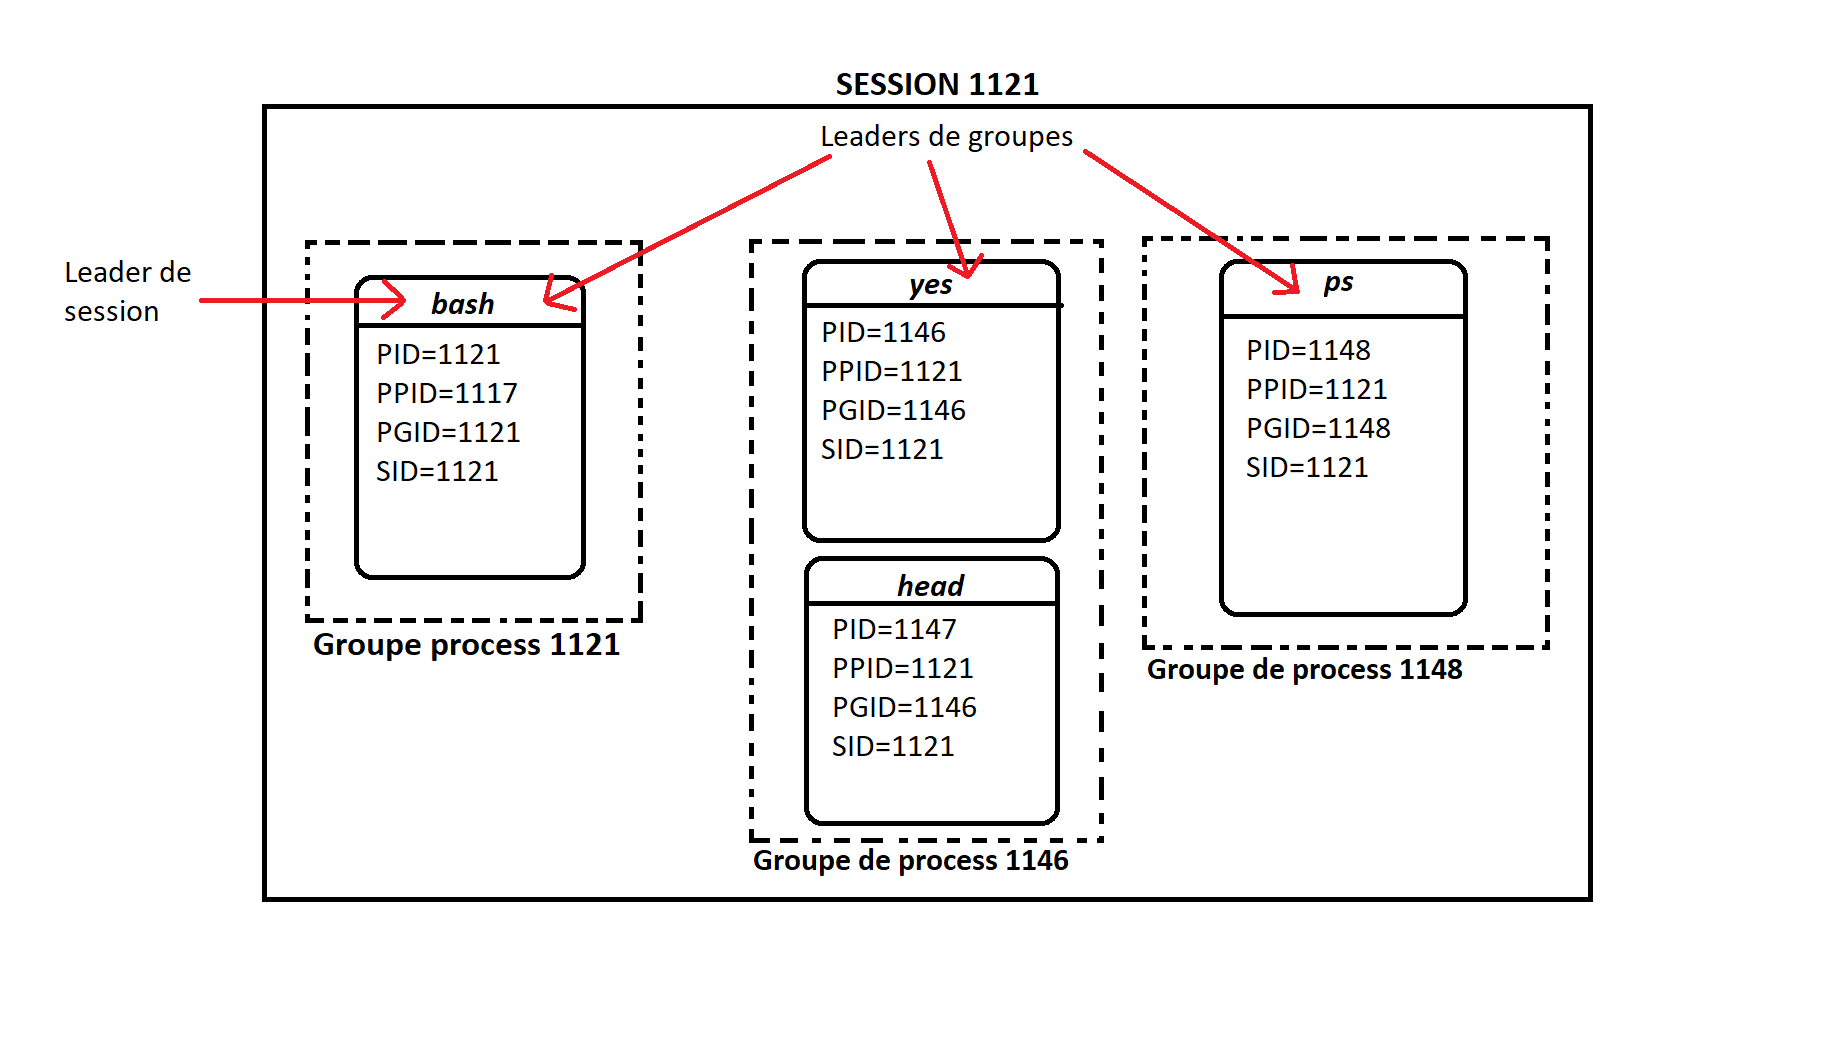
\includegraphics[width=1\textwidth]{img/relationshipSchema.png}
